\section{危险因素辨识与评价}

\subsection{危险因素辨识目的和范围}

根据规范《重大危险源辨识》(GB 18218-2018),所谓重大危险源就是指长期或临时地生产、加工、搬运或贮存危险物质,
且危险物质的数量等于或大于临界量的单元。对于路桥工程施工过程中,对于重大危险源的界定主要包括:
人的危险行为及管理的漏洞、物的不安全的状态、恶劣的环境影响等,由于建筑施工现场的复杂性,工程施工事故可能随时发生,
并可导致人员死亡及伤害、破坏、财产损失,这对于建筑施工工程的整体施工进度已经企业的经济效益都会造成恶劣的影响,
甚至危及企业的发展,因此建筑施工过程中对于重大危险源的辨识、评价和控制,就显得格外重要。

对于重大危险源的辨识,可根据对危险源危险等级的评定方法进行,一般是对施工过程中危险源带来的风险进行评价分析,
根据评价结果又针对性地进行风险控制,从而达到持续改进的目的。常用的风险评价方法有:
作业条件危险性评价法(LEC)、矩阵法、预先危害分析 (PHA)、故障类型及影响分析 (FMEA)、风险概率评价法 (PRA)、危险可操作性研究 (HAZOP)、事故树分析 (ETA) 等等。

\subsection{危险源辨识}
\subsubsection{基坑工程危险源辨识}

\quan{1} 由于未经妥善的土层地质水文勘察而导致的坍塌;

\quan{2} 由于未明确周围既有建筑、地下构筑物、基础平面与周围地下管线的关系而导致的坍塌,触电和其他多重伤害;

\quan{3} 由于深基坑作业人员连续加班、疲劳作业而导致的多重伤害;

\quan{4} 由于基坑降水或围护的抗渗设计未有设计妥善或未按照设计方案施工而导致的坍塌;

\quan{5} 由于夜间作业照明不良而引发的包括物体打击和高处坠落在内的多种伤害;

\quan{6} 由于深基坑未设有临边防护措施而造成的高处坠落和物体打击;

\quan{7} 由于土壤内含有有毒物质而并未提供相应的防护措施而导致的中毒;

\quan{8} 由于水平工作面工作间距不足而造成的包括物体打击,机械伤害和触电在内的多重伤害;

\quan{9} 由于汛期无抗洪措施、冻融期未经特殊处理而导致的坍塌;

\quan{10} 由于施工人员未按设计强度用料或施工导致的坍塌;

\quan{11} 作业人员由于误操作,指挥信号不清或抢工而造成的机械伤害;

\quan{12} 由于桩或桩材料不合规或腐蚀而导致的坍塌或物体打击。

\subsubsection{钢筋工程危险源辨识}

\quan{1} 钢筋加工操作人员未经过相关技术交底和培训,不了解钢筋加工机械的操作方法,导致钢筋加工过程中造成机具伤害;

\quan{2} 钢筋作业人员未取得从业资格证件,无特种作业操作证,在焊接过程中误操作导致触电或者火灾;

\quan{3} 预应力钢筋材料进场未经过检验,导致材料不合格;

\quan{4} 钢筋加工机械未经检验或未按时保养,造成在使用过程中造成触电;

\quan{5} 当使用卷扬机进行冷拉操作时,由于卷扬机固定未有妥善导致被拔出而造成的物体打击;或是卷扬机钢丝绳破损而造成的伤害;

\quan{6} 钢筋切断机锯盘无安全防护导致的机械伤害;

\quan{7} 由于未控制钢筋的冷拉率而造成的的超拉现象,导致机械伤害;

\quan{8} 采用切割机进行切割作业时由于无挡板造成火星飞溅而引起火灾;

\quan{9} 带电操作时未执行“一机一闸一箱一漏”的管理规定而导致储电。

\subsubsection{模板工程危险源辨识}

\quan{1} 由于回填土没压实或压实不到位而造成地基不均匀沉降而导致的模板坍塌;

\quan{2} 由于回填土地基未浇筑硂层或未设置垫板而导致的结构问题或模板坍塌;

\quan{3} 由于立杆、水平杆等支架未按规范搭设而导致的整体支架失稳倒塌;

\quan{4} 由于施工方案与设计方案不符而导致的结构失衡而导致模板或支架倒塌;

\quan{5} 由于构建不齐全而导致的体系坍塌;

\quan{6} 由于模板超载使用,或堆放物过于集中而导致的模板破碎;

\quan{7} 由于违规在模板支架上悬挂起重设备、或是混凝土泵送管搭在模板支架而导致的局部荷载超过设计值而造成模板坍塌;

\quan{8} 高大跨模板搭设是未指定检测方案,或是布置检测点位不足而导致的支撑体系变形,
或是地基不均匀沉降。

\subsubsection{混凝土工程危险源辨识}

\quan{1} 由于运送混凝土时操作人重心失稳或脱把而造成的高处坠落;

\quan{2} 由于运送车道上有杂物而导致的运送推车失稳而造成的高处坠落或物体打击;

\quan{3} 由于运送车道过窄而造成的高处坠落或是物体打击;

\quan{4} 由于泵送混凝土管道架设不规范、不牢靠而导致的机械伤害;

\quan{5} 由于混凝土泵未放置稳妥就开始作业而造成的机械伤害;

\quan{6} 由于作业前未进行试压操作而造成的机械伤害或压力容器爆炸;

\quan{7} 由于乱搭乱接泵送管道或其他工具而造成的储电;

\quan{8} 由于操作工具无接地,无绝缘货物或无漏电保护而造成的触电;

\quan{9} 由于混凝土爆模而导致荷载过于集中而超过最大允许荷载而发生坍塌;

\quan{10} 由于临边洞口未经防护而造成的高处坠落或物体打击。

\subsubsection{脚手架工程危险源辨识}

\quan{1} 由于连墙件未按规定搭设、随意拆除、搭设位置或搭设结构不合理而造成的架体倾倒;

\quan{2} 由于基础发生严重破坏或地基不均匀沉降而造成的架体倾倒;

\quan{3} 由于脚手架设计承载力不足而造成超载而引发的架体倾倒;

\quan{4} 由于脚手架作业成没有铺设妥善脚手板,或者是架体边缘的空隙过大而引发的高处坠落;

\quan{5} 由于作业人员高空抛物而造成的物体打击或是高处坠落;

\quan{6} 脚手架上随意堆放物品而造成的物体打击;

\quan{7} 工人作业未有佩戴防护措施而造成的物体打击或高处坠落。

\subsubsection{吊装作业危险源辨识}

\quan{1} 起重机在运行中对人体造成的挤压或撞击;

\quan{2} 起重机吊钩超载断裂、吊运时钢丝绳从吊钩中滑出;

\quan{3} 吊运中重物坠落造成物体打击,重物从空中落到地面又反弹伤人;

\quan{4} 钢丝绳或麻绳断裂造成重物下落;使用应报废的钢丝绳,使用的吊具吊运超过额定起重量的重物等造成重物下落;

\quan{5} 汽车起重机作业场所地面不平整、支撑不稳定、配重不平衡、重物超过额定起重量而造成起重机倾覆;

\quan{6} 风力过大、违章作业造成起重机倾覆;

\quan{7} 机械传动部分未加防护,造成机械伤害;违章在卷扬机钢丝绳上面通过,运动中的钢丝绳将人挤伤或绊倒;

\quan{8} 载货升降机违章载人;

\quan{9} 人站在起重臂下等危险区域。

\subsubsection{其他危险源辨识}

\quan{1} 由于施工车辆未按照规定走行在内部道路引发的车辆伤害;

\quan{2} 由于作业人员未经培训或未经安全交底而造成的多重伤害;

\quan{3} 由于作业人员在进行动火时未报备项目部,开具动火票而造成的火灾或爆炸;

\quan{4} 由于大型机械作业未有明确的指挥信号而造成的包括物体打击,机械伤害和触电在内的多重伤害;

\quan{5} 雪后未经处理就进场作业而导致的包括车辆伤害和物体打击在内的多重伤害;

\quan{6} 作业工人未有佩戴或未按规定佩戴安全绳而导致的物体打击和高处坠落;

\quan{7} 带电工具未进行绝缘测试就投入使用而引发的触电;

\quan{8} 油漆、涂料和胶水未按规定存放而引起的火灾或中毒;

\quan{9} 由于管理人员违章指挥或指挥失误而引起的多重伤害;

\quan{10} 由于手持机具和金属外壳未进行接地操作而造成的触电;

\quan{11} 由于振捣器工作而产生的震动危害;

\quan{12} 由于易燃易爆物质未经妥善储存而引起的火灾、中毒和窒息、爆炸和压力容器爆炸;

\quan{13} 临边洞口未设置警示标志或未设置防护措施而导致的物体打击或高处坠落;

\quan{14} 高压电未有设置专门的配电箱而引发的火灾或爆炸;

\quan{15} 由于高温,高强度工作,酒后上工等个人因素造成的多重伤害。

\subsection{安全评价}
\subsubsection{评价依据}
\subsubsection{评价目的与评价范围}
\subsubsection{安全评价方法}
\subsubsection{评价单元的划分}
\subsubsection{基坑坍塌事故故障树法安全分析}

造成基坑坍塌事故而造成人员伤亡的情况要同时满足“发生基坑坍塌事故”和“逃生失败”两种情况;发生基坑坍塌事故有可能是设计问题、施工工艺和方法问题,也有可能是现场管理不当;
而逃生失败又分为“无法逃出”和“未察觉有生命危险”。关于基坑坍塌事故的故障树详见图 \ref{fig:c3f1}

\begin{figure}[thbp!]
    \centering
    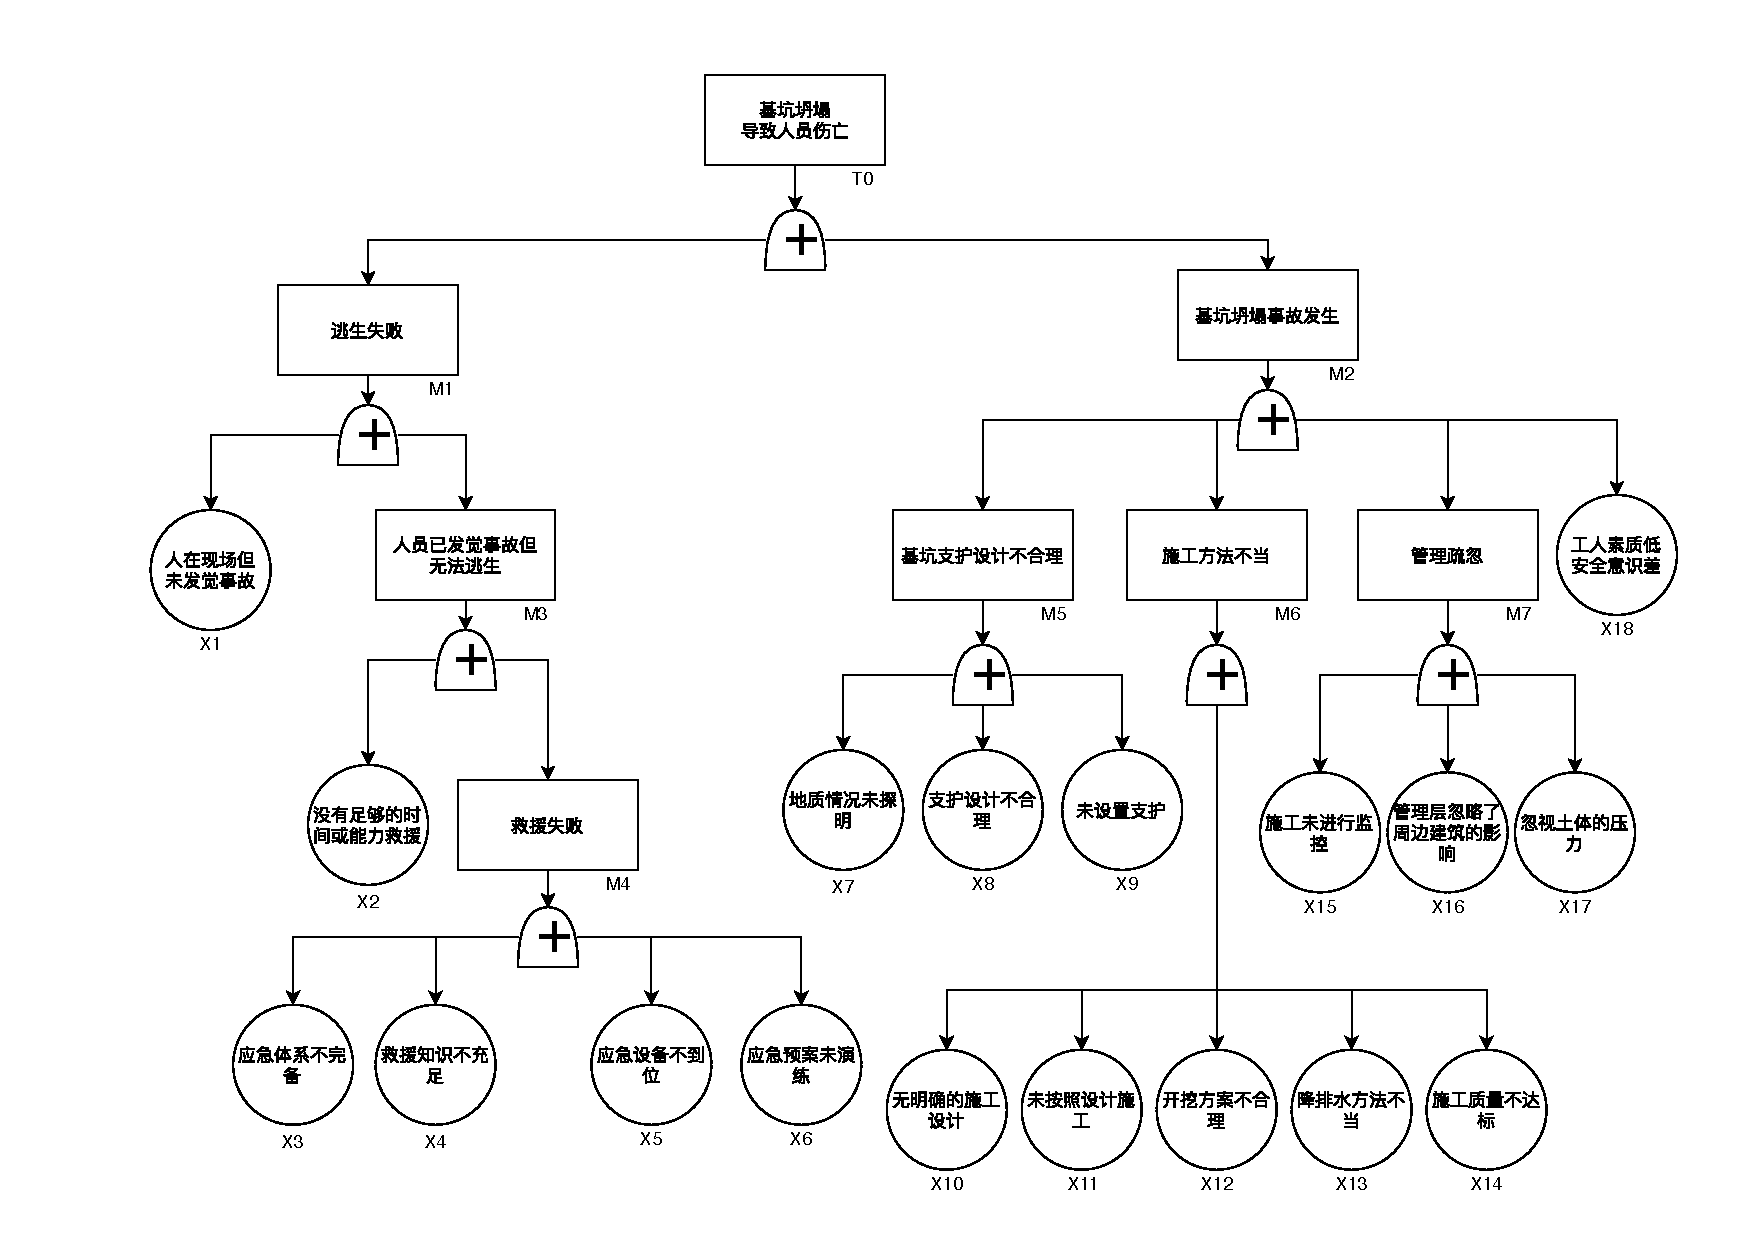
\includegraphics[width=1.0\linewidth]{figure/Untitled Diagram.pdf}
    \caption{基坑坍塌事故树法安全分析}
    \label{fig:c3f1}
\end{figure}

\subsubsection{模板工程坍塌事故故障树法安全分析}
\subsubsection{高处坠落事故故障树法安全分析}
\subsubsection{物料提升机与施工升降机安全检查表法安全分析}

\subsubsection{施工用电安全检查表法安全分析}
\subsubsection{脚手架工程预先危害分析法安全分析}
